\section*{مقدمه}

در این پروژه، هدف ما طراحی و پیاده‌سازی یک سرویس ساده اما قابل اطمینان کلید/مقدار (\lr{Key/Value Server}) با قابلیت کار در محیط‌های شبکه ناپایدار بود. سیستم پیاده‌سازی‌شده باید بتواند تضمین کند که هر درخواست نوشتن حداقل یک بار و حداکثر یک بار روی سرور اجرا شود و از نوشتن دوباره داده‌ها جلوگیری کند. همچنین، این سرویس باید خطی‌سازی‌پذیر (\lr{linearizable}) باشد تا رفتار مشابه یک سرور \lr{single thread} با اجرای ترتیبی درخواست‌ها داشته باشد. در ادامه، مکانیزم قفل توزیع‌شده‌ای نیز روی این سرویس طراحی شد تا چند کلاینت به صورت هماهنگ روی یک ماشین بتوانند به طور همزمان و بدون تضاد به منابع دسترسی داشته باشند.

این پروژه فرصتی بود تا مفاهیم پایه‌ای رایانش توزیع‌شده از جمله \lr{semantics once-most-at}، \lr{linearizability} و پیاده‌سازی قفل توزیع‌شده را به طور عملی تجربه کنیم. همچنین، چالش‌هایی مانند شبکه ناپایدار، گم‌شدن پیام‌ها، تاخیرها و بازفرستادن درخواست‌ها (\lr{retry}) نیز در طراحی و پیاده‌سازی در نظر گرفته شد تا سیستم حاصل، در شرایط واقعی پایدار و قابل اتکا باشد.

\section*{شرح پروژه}

در این پروژه، یک سرور کلید/مقدار ساده طراحی و پیاده‌سازی شد که از طریق فراخوانی‌های \lr{RPC}، کلاینت‌ها قادر به ذخیره‌سازی (\lr{Put}) و بازیابی (\lr{Get}) مقادیر هستند. سرور از یک ساختار \lr{map} در حافظه برای نگهداری جفت‌های کلید-مقدار به همراه ورژن  هر کلید استفاده می‌کند.

هر درخواست \lr{Put} شامل کلید، مقدار و ورژن ارسال می‌شود و تنها در صورتی پذیرفته می‌شود که نسخه ارسالی با نسخه فعلی سرور برای آن کلید مطابقت داشته باشد. این مکانیزم تضمین می‌کند که عملیات نوشتن به صورت اتمیک و متوالی انجام شده و از بازنویسی‌های ناهمزمان جلوگیری شود. همچنین، ورژن هر کلید پس از هر به‌روزرسانی یک واحد افزایش می‌یابد.

برای هماهنگی دسترسی همزمان، در سمت سرور از  \lr{mutex} استفاده شده است تا تنها یک \lr{thread} بتواند همزمان تغییرات روی یک کلید را انجام دهد. این امر باعث می‌شود که سرور رفتار خطی‌سازی‌پذیری را حفظ کند.

در سمت کلاینت، مکانیسم‌های \lr{retry} و \lr{backoff} برای مواجهه با خطاهای احتمالی شبکه و از دست رفتن پیام‌ها پیاده‌سازی شده است. کلاینت‌ها با تولید شناسه‌های یکتا برای هر درخواست \lr{Put} اطمینان حاصل می‌کنند که درخواست‌ها حداکثر یک بار روی سرور اجرا می‌شوند.

بخش بعدی پروژه به پیاده‌سازی قفل توزیع‌شده اختصاص داشت که از سرویس کلید/مقدار به عنوان پایه استفاده می‌کند. این قفل توزیع‌شده به کلاینت‌ها اجازه می‌دهد تا با حفظ قابلیت خطی‌سازی، به صورت ایمن و هماهنگ به منابع مشترک دسترسی داشته باشند. برای این منظور، روش‌هایی مانند شناسه‌گذاری کلاینت‌ها و مکانیزم‌های بازفرستادن درخواست با \lr{backoff} مناسب به کار گرفته شده‌اند.

در نهایت، سیستم طراحی شده با اجرای تست‌های جامع تحت شرایط شبکه‌های قابل اطمینان و ناپایدار مورد ارزیابی قرار گرفت. نتایج تست‌ها نشان داد که سیستم قادر است در شرایط مختلف عملکرد صحیح، هماهنگ و قابل اعتمادی داشته باشد و چالش‌های ناشی از ناپایداری شبکه را به خوبی مدیریت کند.


\section*{توضیحات ساختار کد کلاینت}

در این بخش، به تحلیل ساختار کد کلاینت  پرداخته می‌شود که وظیفه‌ی اصلی آن مدیریت ارتباط با سرور کلید/مقدار از طریق \lr{RPC} است. این کد به‌طور خاص برای پیاده‌سازی دو عملیات اصلی یعنی \lr{Get} و \lr{Put} طراحی شده است.

\subsection*{ساختار کلی کد}

ابتدا، ما یک ساختار \lr{Clerk} تعریف کرده‌ایم که شامل دو فیلد اصلی است:
\begin{itemize}
  \item \lr{clnt}: که یک اشاره‌گر به ساختار \lr{Clnt} از بسته‌ی \lr{tester} است و مسئول مدیریت ارتباطات \lr{RPC} با سرور می‌باشد.
  \item \lr{server}: که آدرس سرور (\lr{string}) را ذخیره می‌کند تا در طول عملیات \lr{Get} و \lr{Put} برای فراخوانی‌ها استفاده شود.
\end{itemize}

ساختار کلاینت به گونه‌ای طراحی شده که از طریق \lr{RPC}، درخواست‌ها را به سرور ارسال کرده و پاسخ‌ها را دریافت می‌کند.

\subsection*{تابع \lr{MakeClerk}}

تابع \lr{MakeClerk} وظیفه‌ی ساخت یک نمونه از \lr{Clerk} را بر عهده دارد و فیلدهای \lr{clnt} و \lr{server} را مقداردهی اولیه می‌کند. در اینجا هیچ منطق اضافی دیگری در نظر گرفته نشده است. به این صورت است که یک کلاینت جدید برای ارتباط با سرور ساخته می‌شود:

\begin{latin}
\begin{lstlisting}[language=Go]
func MakeClerk(clnt *tester.Clnt, server string) kvtest.IKVClerk {
    ck := &Clerk{clnt: clnt, server: server}
    // You may add code here.
    return ck
}
\end{lstlisting}
\end{latin}

تابع \lr{MakeClerk} مسئول ایجاد و مقداردهی اولیه یک نمونه از ساختار \lr{Clerk} است که نماینده‌ی کلاینتی است که می‌خواهد از طریق فراخوانی‌های \lr{RPC} با سرور کلید/مقدار تعامل داشته باشد. این تابع به عنوان نقطه شروع برای استفاده کلاینت در ارتباط با سرور عمل می‌کند و ورودی‌های آن شامل اشاره‌گری به ساختار \lr{Clnt} است که مدیریت ارتباطات \lr{RPC} را بر عهده دارد و همچنین رشته‌ای که آدرس یا شناسه سرور کلید/مقدار را مشخص می‌کند. در این تابع یک نمونه جدید از ساختار \lr{Clerk} ساخته شده و فیلدهای آن شامل \lr{clnt} که مسئول ارتباط \lr{RPC} است و \lr{server} که آدرس سرور را نگهداری می‌کند، مقداردهی اولیه می‌شوند. این تابع صرفاً وظیفه مقداردهی اولیه ساختار کلاینت را دارد و منطق پیچیده‌ای در آن اجرا نمی‌شود، اما در صورت نیاز می‌توان تنظیمات بیشتری مانند تولید شناسه یکتا برای کلاینت یا پارامترهای کمکی دیگر را نیز اضافه کرد. ایجاد این ساختار به کلاینت این امکان را می‌دهد که توابع اصلی \lr{Get} و \lr{Put} را به شکلی سازمان‌دهی شده و ساده برای برقراری ارتباط با سرور استفاده کند و مدیریت درخواست‌ها و پاسخ‌ها را به طور مؤثر انجام دهد.


\subsection*{تابع \lr{Get}}

تابع \lr{Get} مسئول دریافت مقدار و نسخه جاری یک کلید از سرور است. این تابع از پروسه‌ی \lr{RPC} برای فراخوانی متد \lr{KVServer.Get} روی سرور استفاده می‌کند. کد این تابع به‌طور دائمی در تلاش است تا با سرور ارتباط برقرار کند و در صورت دریافت خطا یا عدم دریافت پاسخ، درخواست را مجدداً ارسال می‌کند.

این تابع به‌صورت زیر عمل می‌کند:
\begin{itemize}
  \item ابتدا، ساختار \lr{GetArgs} حاوی کلید مورد نظر ایجاد شده و به سرور ارسال می‌شود.
  \item سپس با استفاده از تابع \lr{Call}، درخواست \lr{RPC} به سرور ارسال می‌شود.
  \item اگر درخواست با موفقیت ارسال شد یا اگر کلید مورد نظر در سرور موجود نباشد (\lr{ErrNoKey})، حلقه خاتمه می‌یابد.
  \item در صورت بروز خطاهای دیگر، تابع یک وقفه زمانی (\lr{time.Sleep}) اعمال کرده و دوباره درخواست را ارسال می‌کند.
\end{itemize}

این مکانیزم \lr{retry} به‌طور خاص برای مقابله با خطاهای موقتی و مشکلات شبکه طراحی شده است.

\begin{latin}
\begin{lstlisting}[language=Go]
func (ck *Clerk) Get(key string) (string, rpc.Tversion, rpc.Err) {
    args := rpc.GetArgs{Key: key}
    reply := rpc.GetReply{}

    for {
        ok := ck.clnt.Call(ck.server, "KVServer.Get", &args, &reply)
        if ok || (reply.Err == rpc.ErrNoKey) {
            break
        }
        time.Sleep(100 * time.Millisecond)
    }

    return reply.Value, reply.Version, reply.Err
}
\end{lstlisting}
\end{latin}

\subsection*{تابع \lr{Put}}

تابع \lr{Put} مسئول به‌روزرسانی مقدار کلید در سرور است. برای انجام این کار، نسخه  دریافتی از درخواست با نسخه فعلی کلید در سرور مقایسه می‌شود. اگر نسخه‌ها مطابقت داشته باشند، مقدار جدید نوشته می‌شود. در صورتی که نسخه‌ها مطابقت نداشته باشند، سرور باید خطای \lr{ErrVersion} را برگرداند.

منطق تابع به این صورت است:
\begin{itemize}
  \item ابتدا، ساختار \lr{PutArgs} شامل کلید، مقدار و نسخه ارسال می‌شود.
  \item درخواست \lr{RPC} به سرور ارسال شده و نتیجه در ساختار \lr{PutReply} ذخیره می‌شود.
  \item اگر درخواست به موفقیت انجام نشود و خطای \lr{ErrVersion} دریافت شود، تابع \lr{ErrMaybe} را به برنامه بازمی‌گرداند تا نشان دهد که عملیات ممکن است در سرور انجام شده باشد ولی پاسخ گم شده است.
  \item در صورت دریافت خطاهای دیگر، درخواست دوباره ارسال می‌شود.
\end{itemize}

این تابع از مکانیزم \lr{retry} و \lr{backoff} برای مقابله با مشکلات شبکه و گم شدن پاسخ‌ها استفاده می‌کند.

\begin{latin}
\begin{lstlisting}[language=Go]
func (ck *Clerk) Put(key, value string, version rpc.Tversion) rpc.Err {

    args := rpc.PutArgs{Key: key, Value: value, Version: version}
    reply := rpc.PutReply{}

    ok := ck.clnt.Call(ck.server, "KVServer.Put", &args, &reply)

    for !ok {
        ok = ck.clnt.Call(ck.server, "KVServer.Put", &args, &reply)
        if reply.Err == rpc.ErrVersion {
            return rpc.ErrMaybe
        }
        time.Sleep(100 * time.Millisecond)
    }
    return reply.Err
}
\end{lstlisting}
\end{latin}


تابع \lr{Put} و \lr{Get} دو عملکرد اصلی سیستم کلید/مقدار هستند که به‌طور مستقیم با سرور ارتباط برقرار کرده و عملیات ذخیره‌سازی و بازیابی داده‌ها را انجام می‌دهند. تابع \lr{Get} با استفاده از مکانیزم \lr{retry} اطمینان می‌دهد که حتی در صورت بروز خطاهای موقت، درخواست به سرور ارسال می‌شود. تابع \lr{Put} نیز با مدیریت نسخه‌ها و استفاده از مکانیزم \lr{ErrVersion} و \lr{ErrMaybe} اطمینان می‌دهد که داده‌ها به‌طور صحیح و یک‌بار در سرور ذخیره می‌شوند.

این منطق و ساختار طراحی، به‌ویژه در شرایط ناپایدار شبکه، از مشکلاتی مانند گم شدن پیام‌ها، \lr{retry} و اطمینان از یکسان بودن نسخه‌ها جلوگیری می‌کند و سیستم را در برابر خطاها مقاوم می‌سازد.


\section*{توضیحات ساختار کد سرور \lr{KVServer}}

در این بخش، به تحلیل ساختار کد سرور \lr{KVServer} پرداخته می‌شود که به‌عنوان هسته‌ی اصلی سیستم کلید/مقدار طراحی و پیاده‌سازی شده است. این سرور وظیفه مدیریت داده‌های کلید/مقدار را بر عهده دارد و از مکانیزم‌های همزمانی برای جلوگیری از دسترسی همزمان و ناخواسته به داده‌ها استفاده می‌کند. در این توضیحات، ابتدا ساختار کلی کد بررسی می‌شود و سپس به تفصیل به هر یک از توابع سرور پرداخته خواهد شد. سرور پیاده‌سازی‌شده دو عملیات اصلی \lr{Get} و \lr{Put} را برای بازیابی و ذخیره‌سازی داده‌ها انجام می‌دهد و برای همزمانی و جلوگیری از مشکلات رقابتی از قفل‌ها \lr{mutex} استفاده می‌کند.

\subsection*{ساختار کلی کد}

در ابتدا، یک ساختار \lr{Record} تعریف شده است که به‌عنوان واحد ذخیره‌سازی داده‌ها در سرور عمل می‌کند. این ساختار به‌گونه‌ای طراحی شده است که دو فیلد اصلی برای ذخیره‌سازی داده‌ها دارد:
\begin{itemize}
  \item \lr{Value}: این فیلد مقدار واقعی داده‌ای است که برای کلید مشخص شده ذخیره می‌شود. مقدار داده‌ها به‌صورت رشته ذخیره می‌شود.
  \item \lr{Version}: این فیلد برای نگهداری نسخه داده استفاده می‌شود. هر بار که داده به‌روزرسانی می‌شود، نسخه‌ی آن افزایش می‌یابد تا از تداخل داده‌ها در فرآیندهای مختلف جلوگیری شود.
\end{itemize}

پس از تعریف ساختار \lr{Record}، ساختار اصلی \lr{KVServer} تعریف می‌شود که وظیفه مدیریت داده‌ها را بر عهده دارد. این ساختار از یک \lr{map} به نام \lr{records} استفاده می‌کند که جفت‌های کلید-مقدار را ذخیره می‌کند. \lr{map} به‌طور مؤثر به سرور این امکان را می‌دهد که داده‌ها را ذخیره کرده و به‌راحتی به آن‌ها دسترسی پیدا کند. همچنین، برای جلوگیری از مشکلات همزمانی در دسترسی به داده‌ها و برای جلوگیری از دسترسی همزمان به داده‌ها توسط چندین کلاینت، یک قفل به نام \lr{mu} از نوع \lr{sync.Mutex} به این ساختار اضافه شده است.

این قفل به‌گونه‌ای عمل می‌کند که در هر زمان تنها یک کلاینت می‌تواند به داده‌ها دسترسی پیدا کند. از این طریق، عملیات همزمان به داده‌ها مدیریت شده و از مشکلات رقابتی جلوگیری می‌شود. در نهایت، برای ایجاد یک نمونه از سرور، تابع \lr{MakeKVServer} استفاده می‌شود که یک نمونه جدید از \lr{KVServer} را می‌سازد و فضای لازم برای ذخیره‌سازی جفت‌های کلید-مقدار را تخصیص می‌دهد.

\begin{latin}
\begin{lstlisting}[language=Go]
type Record struct {
    Value   string
    Version rpc.Tversion
}

type KVServer struct {
    mu      sync.Mutex
    records map[string]*Record
}

func MakeKVServer() *KVServer {
    kv := &KVServer{}
    kv.records = make(map[string]*Record)
    return kv
}
\end{lstlisting}
\end{latin}

در این کد، از قفل‌های \lr{sync.Mutex} برای همزمانی استفاده می‌شود تا دسترسی به داده‌ها به‌طور ایمن و بدون تداخل انجام شود. همچنین از \lr{map} برای ذخیره‌سازی داده‌ها استفاده می‌شود که به سرور اجازه می‌دهد به‌راحتی داده‌ها را ذخیره کرده و به آن‌ها دسترسی داشته باشد.

\subsection*{تابع \lr{Get}}

تابع \lr{Get} وظیفه بازیابی مقدار و نسخه یک کلید از سرور را بر عهده دارد. این تابع ابتدا بررسی می‌کند که آیا کلید مورد نظر در \lr{map} موجود است یا خیر. اگر کلید موجود نباشد، خطای \lr{ErrNoKey} به پاسخ ارسال می‌شود. در غیر این صورت، مقدار و نسخه کلید به همراه خطای \lr{OK} به کلاینت ارسال می‌شود. این کار باعث می‌شود که در صورت نبودن داده‌ی مورد نظر، پاسخ مناسبی به کلاینت ارسال شود.

عملکرد این تابع به‌گونه‌ای است که ابتدا با استفاده از \lr{mu.Lock} قفل می‌شود تا از دسترسی همزمان به داده‌ها جلوگیری شود. سپس در صورتی که کلید موجود باشد، داده‌ها از \lr{map} استخراج می‌شوند و به کلاینت بازمی‌گردند. در غیر این صورت، خطا \lr{ErrNoKey} به کلاینت ارسال می‌شود. پس از اتمام عملیات، با استفاده از \lr{defer kv.mu.Unlock()} قفل آزاد می‌شود.

\begin{latin}
\begin{lstlisting}[language=Go]
func (kv *KVServer) Get(args *rpc.GetArgs, reply *rpc.GetReply) {
    kv.mu.Lock()
    defer kv.mu.Unlock()

    record, ok := kv.records[args.Key]
    if !ok {
        reply.Err = rpc.ErrNoKey
        return
    }

    reply.Err = rpc.OK
    reply.Version = record.Version
    reply.Value = record.Value
}
\end{lstlisting}
\end{latin}

در این کد، از \lr{mu.Lock} برای قفل‌کردن داده‌ها و جلوگیری از دسترسی همزمان به آن‌ها استفاده می‌شود و پس از اتمام عملیات، با \lr{defer} قفل آزاد می‌شود.

\subsection*{تابع \lr{Put}}

تابع \lr{Put} مسئول به‌روزرسانی یا درج مقدار جدید برای یک کلید است. این تابع ابتدا با استفاده از \lr{mutex} برای جلوگیری از همزمانی، دسترسی به نقشه داده‌ها را کنترل می‌کند. سپس، بر اساس وضعیت نسخه‌ها، تصمیم می‌گیرد که چه عملیاتی انجام دهد:
\begin{itemize}
  \item اگر کلید موجود نباشد و نسخه ارسال‌شده صفر باشد، یک رکورد جدید با نسخه 1 ساخته می‌شود.
  \item اگر کلید موجود نباشد و نسخه ارسال‌شده غیر از صفر باشد، خطای \lr{ErrNoKey} ارسال می‌شود.
  \item اگر نسخه‌های کلید موجود و نسخه ارسال‌شده تطابق داشته باشد، مقدار به‌روزرسانی شده و نسخه آن افزایش می‌یابد.
  \item اگر نسخه‌ها تطابق نداشته باشند، خطای \lr{ErrVersion} ارسال می‌شود.
\end{itemize}

این طراحی باعث می‌شود که داده‌ها به‌صورت همزمان و بدون تضاد در سرور به‌روزرسانی شوند. همچنین از مکانیزم \lr{mutex} برای هماهنگ کردن دسترسی به داده‌ها و جلوگیری از تضاد در تغییرات استفاده می‌شود.

\begin{latin}
\begin{lstlisting}[language=Go]
func (kv *KVServer) Put(args *rpc.PutArgs, reply *rpc.PutReply) {
    kv.mu.Lock()
    defer kv.mu.Unlock()

    record, exists := kv.records[args.Key]
    switch {
    case !exists && args.Version == 0:
        kv.records[args.Key] = &Record{
            Value:   args.Value,
            Version: 1,
        }
        reply.Err = rpc.OK

    case !exists:
        reply.Err = rpc.ErrNoKey

    case record.Version == args.Version:
        record.Value = args.Value
        record.Version++
        reply.Err = rpc.OK

    default:
        reply.Err = rpc.ErrVersion
    }
}
\end{lstlisting}
\end{latin}

در این کد، به‌طور واضح از \lr{mu.Lock} و \lr{defer kv.mu.Unlock()} استفاده می‌شود تا قفل تنها برای مدت زمان لازم نگه داشته شود و بعد از انجام عملیات قفل آزاد شود. همچنین با استفاده از \lr{switch} و بررسی نسخه‌ها، به‌طور دقیق مدیریت می‌شود که چه زمانی مقدار کلید باید به‌روزرسانی شود.

\subsection*{تابع \lr{Kill}}

تابع \lr{Kill} در این پیاده‌سازی نادیده گرفته شده است. این تابع برای متوقف کردن سرور طراحی شده است، اما چون هدف این پروژه تمرکز بر پیاده‌سازی اولیه سرور است و قابلیت‌های مربوط به شبیه‌سازی سرورهای افزونه‌ای و مکرر (\lr{replicated}) مدنظر نبوده، این تابع در کد نهایی وجود ندارد.

\begin{latin}
\begin{lstlisting}[language=Go]
func (kv *KVServer) Kill() {
}
\end{lstlisting}
\end{latin}

\subsection*{تابع \lr{StartKVServer}}

تابع \lr{StartKVServer} برای راه‌اندازی سرور و آماده‌سازی آن برای ارتباط با کلاینت‌ها از طریق \lr{RPC} طراحی شده است. این تابع یک نمونه از \lr{KVServer} می‌سازد و آن را به‌عنوان سرویس در دسترس قرار می‌دهد. این تابع همچنین به‌طور ساده سرور را برای برقراری ارتباط با کلاینت‌ها از طریق \lr{RPC} آماده می‌کند و برای شروع به‌کار آن نیاز به هیچ‌گونه پارامتر یا ورودی اضافی ندارد.

\begin{latin}
\begin{lstlisting}[language=Go]
func StartKVServer(ends []*labrpc.ClientEnd, gid tester.Tgid, srv int, persister *tester.Persister) []tester.IService {
    kv := MakeKVServer()
    return []tester.IService{kv}
}
\end{lstlisting}
\end{latin}

در این کد، تنها یک سرور جدید ساخته می‌شود و به‌عنوان سرویس برای پذیرش درخواست‌های \lr{RPC} آماده می‌شود. این تابع هیچ‌گونه پیچیدگی اضافی ندارد و به‌سادگی سرور را راه‌اندازی می‌کند.


کد پیاده‌سازی‌شده برای سرور \lr{KVServer} به‌طور مؤثر وظایف اصلی خود را برای مدیریت داده‌های کلید/مقدار با استفاده از مکانیزم‌های همزمانی انجام می‌دهد. این سرور از قفل‌ها برای جلوگیری از مشکلات همزمانی استفاده می‌کند و با استفاده از نسخه‌ها، از بروز تضاد در هنگام به‌روزرسانی داده‌ها جلوگیری می‌کند. طراحی ساده و کارآمد این سرور باعث می‌شود که بتواند به‌خوبی در شرایط مختلف به‌ویژه در شبکه‌های توزیع‌شده با قابلیت اطمینان محدود عمل کند.

\section*{توضیحات ساختار کد \lr{lock}}

در این بخش، قصد داریم به تحلیل ساختار کد \lr{Lock} بپردازیم که به‌طور خاص مسئول پیاده‌سازی یک قفل توزیع‌شده برای مدیریت همزمانی دسترسی به منابع مشترک در سیستم کلید/مقدار است. در این سیستم، از سرویس کلید/مقدار استفاده می‌کنیم تا حالت قفل را در سرور ذخیره کرده و مدیریت کنیم. هدف اصلی این قفل این است که در شرایط همزمانی، فقط یک کلاینت در هر زمان بتواند به منابع مشترک دسترسی داشته باشد و سایر کلاینت‌ها باید تا آزاد شدن قفل منتظر بمانند.

\subsection*{ساختار کلی کد}

در ابتدا، ساختار \lr{Lock} تعریف شده است که شامل چندین فیلد مهم است:
\begin{itemize}
  \item \lr{ck}: این فیلد یک اشاره‌گر به \lr{IKVClerk} است که مسئول برقراری ارتباط با سیستم کلید/مقدار می‌باشد. با استفاده از این ساختار، می‌توانیم عملیات‌های \lr{Put} و \lr{Get} را انجام دهیم.
  \item \lr{clientId}: شناسه یکتای هر کلاینت است که برای شناسایی و تعیین مالک قفل به کار می‌رود. به عبارت دیگر، این شناسه کلاینت‌ها را از هم متمایز کرده و اطمینان حاصل می‌کند که هر کلاینت فقط قفل‌هایی را که خود دریافت کرده، آزاد کند.
  \item \lr{lockKey}: کلید منحصر به‌فردی است که وضعیت قفل در آن ذخیره می‌شود. این کلید به‌طور خاص برای نگهداری اطلاعات مربوط به وضعیت قفل در سرور استفاده می‌شود.
  \item \lr{mu}: این فیلد یک \lr{mutex} است که برای مدیریت همزمانی و جلوگیری از مشکلات رقابتی در دسترسی به منابع مشترک مورد استفاده قرار می‌گیرد. این \lr{mutex} از این جهت اهمیت دارد که اطمینان حاصل می‌کند که هیچ دو کلاینتی به طور همزمان نتوانند تغییرات همزمانی در وضعیت قفل اعمال کنند.
\end{itemize}

این ساختار وظیفه مدیریت قفل‌ها را بر عهده دارد و به هر کلاینت این امکان را می‌دهد که برای گرفتن یا آزاد کردن قفل از آن استفاده کند. به عبارت دیگر، قفل‌ها برای جلوگیری از دسترسی همزمان و تضاد بین درخواست‌ها در سیستم طراحی شده‌اند.

\begin{latin}
\begin{lstlisting}[language=Go]
type Lock struct {
    ck       kvtest.IKVClerk
    clientId string
    lockKey  string
    mu       sync.Mutex
}
\end{lstlisting}
\end{latin}

\subsection*{تابع \lr{MakeLock}}

تابع \lr{MakeLock} مسئول ساخت یک نمونه جدید از \lr{Lock} است. این تابع دو ورودی دریافت می‌کند: یک کلاینت (\lr{ck}) و یک کلید (\lr{lockKey}). با استفاده از این ورودی‌ها، یک قفل جدید ایجاد می‌شود. علاوه بر این، در این تابع شناسه یکتای کلاینت به‌طور تصادفی از طریق تابع \lr{kvtest.RandValue} تولید می‌شود تا هر کلاینت شناسه‌ای منحصر به‌فرد برای خود داشته باشد.

این تابع تنها قفل جدید را ایجاد کرده و مقادیر اولیه را تنظیم می‌کند. پس از ساخت قفل، آن را برای استفاده در سایر قسمت‌های کد باز می‌گرداند.

\begin{latin}
\begin{lstlisting}[language=Go]
func MakeLock(ck kvtest.IKVClerk, l string) *Lock {
    lk := &Lock{
        ck:       ck,
        lockKey:  l,
        clientId: kvtest.RandValue(8),
    }
    return lk
}
\end{lstlisting}
\end{latin}

\subsection*{تابع \lr{Acquire}}

تابع \lr{Acquire} مسئول گرفتن قفل از سرور است. در این تابع، ابتدا بررسی می‌شود که آیا قفل در حال حاضر متعلق به کلاینت است یا خیر. اگر قفل در دسترس باشد (یعنی قفل قبلاً گرفته نشده باشد یا برای این کلاینت باشد)، کلاینت می‌تواند به‌راحتی قفل را بگیرد. در غیر این صورت، کلاینت باید منتظر بماند تا قفل توسط کلاینت دیگر آزاد شود.

در این تابع، ابتدا با استفاده از تابع \lr{Get} وضعیت قفل بررسی می‌شود. اگر مقدار موجود در قفل برابر با شناسه کلاینت باشد، یعنی قفل قبلاً توسط این کلاینت گرفته شده است و نیازی به تغییر آن نیست. در غیر این صورت، تابع سعی می‌کند با استفاده از تابع \lr{Put} شناسه خود را به‌عنوان صاحب قفل در سرور ذخیره کند.

همچنین برای جلوگیری از تداخل دسترسی به منابع و مشکلات همزمانی، از \lr{mutex} استفاده شده است. این \lr{mutex} به‌طور مؤثر دسترسی به منابع را مدیریت می‌کند و اطمینان حاصل می‌کند که فقط یک کلاینت در هر زمان تغییرات روی قفل را انجام دهد.

در صورت بروز هرگونه خطا (مانند گم شدن پیام‌ها یا تأخیر در پردازش)، تابع به‌طور خودکار تلاش مجدد انجام می‌دهد و تا زمانی که قفل به‌دست نیامده باشد، عملیات را تکرار می‌کند.

\begin{latin}
\begin{lstlisting}[language=Go]
func (lk *Lock) Acquire() {
    i := 100
    for {
        lk.mu.Lock()
        val, version, err := lk.ck.Get(lk.lockKey)

        if val == lk.clientId {
            lk.mu.Unlock()
            return
        }

        if err == rpc.ErrNoKey || (err == rpc.OK && val == "") {
            err = lk.ck.Put(lk.lockKey, lk.clientId, version)
            if err == rpc.OK {
                lk.mu.Unlock()
                return
            }
        }

        lk.mu.Unlock()
        time.Sleep(time.Duration(i) * time.Millisecond)
        i += 10
    }
}
\end{lstlisting}
\end{latin}

در اینجا، علاوه بر استفاده از \lr{mutex} برای مدیریت همزمانی، از \lr{retry} و \lr{backoff} نیز استفاده می‌شود. این مکانیزم به ما کمک می‌کند که در صورت مواجهه با مشکلات شبکه، بتوانیم درخواست را دوباره ارسال کرده و از بروز خطاهای موقتی جلوگیری کنیم.

\subsection*{تابع \lr{Release}}

تابع \lr{Release} برای آزاد کردن قفل از سرور استفاده می‌شود. در اینجا، ابتدا با استفاده از تابع \lr{Get} بررسی می‌شود که آیا قفل به این کلاینت تعلق دارد یا خیر. اگر قفل متعلق به کلاینت باشد، با استفاده از \lr{Put} مقدار کلید به‌صورت خالی ذخیره می‌شود تا قفل آزاد شود. در غیر این صورت، تابع تلاش می‌کند که دوباره عملیات \lr{Release} را انجام دهد.

مانند تابع \lr{Acquire}، در اینجا نیز از \lr{mutex} برای همزمانی استفاده شده است تا اطمینان حاصل شود که هیچ‌گونه تضاد یا تداخل در دسترسی به منابع وجود ندارد.

در این تابع هم از مکانیزم \lr{retry} برای مقابله با مشکلات احتمالی مانند گم شدن پیام‌ها یا تأخیرهای شبکه استفاده می‌شود.

\begin{latin}
\begin{lstlisting}[language=Go]
func (lk *Lock) Release() {
    i := 100
    for {
        lk.mu.Lock()
        value, version, err := lk.ck.Get(lk.lockKey)

        if err == rpc.OK && value == lk.clientId {
            lk.ck.Put(lk.lockKey, "", version)
            lk.mu.Unlock()
            break
        }

        lk.mu.Unlock()
        time.Sleep(time.Duration(i) * time.Millisecond)
        i += 10
    }
}
\end{lstlisting}
\end{latin}

کد قفل توزیع‌شده‌ای که طراحی کرده‌ایم به‌طور مؤثر و کارآمد مدیریت قفل‌ها را در یک سیستم توزیع‌شده با استفاده از سیستم کلید/مقدار انجام می‌دهد. این سیستم به‌گونه‌ای طراحی شده که در برابر خطاهای شبکه و همزمانی دسترسی به منابع از طریق مکانیزم‌های \lr{retry} و \lr{backoff} مقاوم باشد. به‌طور کلی، این سیستم به هر کلاینت این امکان را می‌دهد که به‌صورت ایمن و هماهنگ به منابع مشترک دسترسی داشته باشد و در شرایطی که چندین کلاینت بخواهند به یک منبع دسترسی داشته باشند، از بروز تضاد و تداخل جلوگیری می‌کند.

این طراحی ساده اما مؤثر از روش‌های قفل توزیع‌شده و همزمانی برای جلوگیری از مشکلات همزمانی و تداخل در دسترسی به منابع استفاده می‌کند. به‌ویژه در شرایط ناپایدار شبکه، این سیستم با استفاده از مکانیزم‌های بازفرستادن درخواست (\lr{retry}) و تأخیر (\lr{backoff}) توانسته است عملکرد خود را به‌طور صحیح و بدون هیچ‌گونه مشکل حفظ کند.

این سیستم علاوه بر ساده بودن، بسیار مؤثر است و توانایی دارد در برابر خطاهای احتمالی و شرایط رقابتی پیچیده‌ای که در محیط‌های توزیع‌شده وجود دارد، ایمن باقی بماند.

\section*{توضیحات ساختار کد \lr{TestKV}}

در این بخش به تحلیل ساختار کد مربوط به اجرای تست‌های سامانه کلید/مقدار (\lr{Key/Value}) می‌پردازیم. این بخش از کد وظیفه راه‌اندازی، مدیریت و اجرای تست‌ها در دو حالت شبکه قابل اطمینان و ناپایدار را بر عهده دارد و به منظور ارزیابی عملکرد سیستم کلید/مقدار طراحی شده است.

\subsection*{ساختار کلی کد}

در ابتدا ساختار \lr{TestKV} تعریف شده که شامل سه فیلد اصلی است:

\begin{itemize}
  \item \texttt{kvtest.Test}: اشاره‌گری به ساختار \lr{Test} که نمایانگر مجموعه‌ای از ابزارها و داده‌های مرتبط با اجرای یک تست کلی است.
  \item \texttt{t testing.T}: اشاره‌گری به ساختار \lr{testing.T} در زبان \lr{Go} که برای مدیریت و گزارش نتایج تست‌ها به کار می‌رود.
  \item \texttt{reliable bool}: متغیری بولی که تعیین می‌کند تست‌ها در محیط شبکه قابل اطمینان \lr{true} یا ناپایدار \lr{false} اجرا شوند.
\end{itemize}

این ساختار به عنوان لایه‌ای مدیریتی برای تنظیم و کنترل تست‌ها عمل کرده و اطلاعات مربوط به نوع تست و محیط اجرای آن را ذخیره می‌کند.

\begin{latin}
\begin{lstlisting}[language=Go]
type TestKV struct {
    *kvtest.Test
    t        *testing.T
    reliable bool
}
\end{lstlisting}
\end{latin}

\subsection*{تابع \lr{MakeTestKV}}

این تابع مسئول ایجاد یک نمونه جدید از \lr{TestKV} است که برای اجرای تست‌ها به کار می‌رود. روند عملکرد این تابع به شرح زیر است:

\begin{itemize}
  \item با فراخوانی تابع \lr{tester.MakeConfig}، یک کانفیگ برای تست ساخته می‌شود که تعداد سرورها، نوع شبکه (قابل اطمینان یا ناپایدار) و تابع شروع سرور را دریافت می‌کند.
  \item سپس یک نمونه جدید از \lr{TestKV} ساخته شده و فیلدهای \lr{t} و \lr{reliable} مقداردهی می‌شوند.
  \item در نهایت با فراخوانی \lr{kvtest.MakeTest} تست اصلی ایجاد شده و به فیلد \lr{Test} اختصاص داده می‌شود تا این ساختار بتواند به تمام امکانات اجرای تست‌ها دسترسی داشته باشد.
  \item نمونه ایجاد شده بازگردانده می‌شود تا در اجرای تست‌ها استفاده شود.
\end{itemize}

\begin{latin}
\begin{lstlisting}[language=Go]
func MakeTestKV(t *testing.T, reliable bool) *TestKV {
    cfg := tester.MakeConfig(t, 1, reliable, StartKVServer)
    ts := &TestKV{
        t:        t,
        reliable: reliable,
    }
    ts.Test = kvtest.MakeTest(t, cfg, false, ts)
    return ts
}
\end{lstlisting}
\end{latin}

\subsection*{تابع \lr{MakeClerk}}

این تابع برای ساخت یک کلاینت جدید در چارچوب تست به کار می‌رود. کلاینت وظیفه ارسال درخواست‌های \lr{Put} و \lr{Get} را به سرور کلید/مقدار بر عهده دارد. نحوه عملکرد آن به شرح زیر است:

\begin{itemize}
  \item ابتدا با استفاده از کانفیگ موجود در \lr{TestKV}، کلاینتی جدید ساخته می‌شود که قادر به برقراری ارتباط با سرور است.
  \item سپس با فراخوانی تابع \lr{MakeClerk}، یک کلاینت سطح بالاتر ساخته می‌شود که آدرس مشخصی از سرور (سرور شماره صفر در گروه صفر) به آن داده شده است.
  \item این کلاینت ساخته شده در قالب یک \lr{TestClerk} بسته‌بندی شده و به عنوان خروجی بازگردانده می‌شود تا در تست‌ها مورد استفاده قرار گیرد.
\end{itemize}

\begin{latin}
\begin{lstlisting}[language=Go]
func (ts *TestKV) MakeClerk() kvtest.IKVClerk {
    clnt := ts.Config.MakeClient()
    ck := MakeClerk(clnt, tester.ServerName(tester.GRP0, 0))
    return &kvtest.TestClerk{ck, clnt}
}
\end{lstlisting}
\end{latin}

\subsection*{تابع \lr{DeleteClerk}}

در پایان استفاده از کلاینت، این تابع برای حذف کلاینت ایجاد شده و آزادسازی منابع مربوطه استفاده می‌شود. عملکرد آن شامل:

\begin{itemize}
  \item تبدیل نمونه کلاینت عمومی (\lr{IKVClerk}) به نوع اختصاصی \lr{TestClerk} انجام می‌شود تا بتوان به ساختار داخلی آن دسترسی داشت.
  \item سپس کلاینت با فراخوانی تابع \lr{DeleteClient} از سیستم حذف و منابع مرتبط آزاد می‌شوند.
\end{itemize}

این کار باعث می‌شود که کلاینت‌ها به صورت منظم مدیریت شده و از نشت منابع جلوگیری شود.

\begin{latin}
\begin{lstlisting}[language=Go]
func (ts *TestKV) DeleteClerk(ck kvtest.IKVClerk) {
    tck := ck.(*kvtest.TestClerk)
    ts.DeleteClient(tck.Clnt)
}
\end{lstlisting}
\end{latin}

\section*{نتایج اجرای تست‌های خودکار}

 این تست‌ها شامل بررسی عملکرد سیستم در شرایط شبکه قابل اطمینان و ناپایدار در دو بخش اصلی هستند: تست‌های سرویس کلید/مقدار و تست‌های قفل توزیع‌شده.

\subsection*{تست‌های سرویس کلید/مقدار}

\subsubsection*{1. تست سرویس کلید/مقدار در شرایط شبکه قابل اطمینان (\texttt{TestOneClientReliable} و \texttt{TestManyClientsReliable})}

این تست‌ها اطمینان حاصل می‌کنند که سرویس کلید/مقدار در شرایط شبکه قابل اطمینان به درستی عمل می‌کند. در این شرایط، شبکه به‌طور پایدار عمل می‌کند و پیام‌ها بدون مشکل به سرور ارسال می‌شوند و پاسخ‌ها به درستی برگشت داده می‌شوند. هدف از این تست‌ها بررسی موارد زیر است:
\begin{itemize}
    \item \textbf{درخواست‌های \texttt{Put} و \texttt{Get}:} این تست‌ها بررسی می‌کنند که آیا سرور به درستی درخواست‌های \texttt{Put} و \texttt{Get} را پردازش کرده و داده‌ها را ذخیره یا بازیابی می‌کند.
    \item \textbf{ذخیره‌سازی و بازیابی داده‌ها:} اطمینان از اینکه داده‌ها به درستی ذخیره و بازیابی می‌شوند، یعنی پس از ذخیره‌سازی یک مقدار توسط کلاینت، هنگام درخواست از سرور همان مقدار برگشت داده شود.
    \item \textbf{ارتباطات صحیح میان کلاینت و سرور:} در این تست‌ها، رفتار ارتباطی میان کلاینت‌ها و سرور در شرایط پایدار شبکه بررسی می‌شود و از صحت برقراری ارتباط اطمینان حاصل می‌شود.
\end{itemize}

\subsubsection*{2. تست سرویس کلید/مقدار در شرایط شبکه ناپایدار (\texttt{TestOneClientUnreliable} و \texttt{TestManyClientsUnreliable})}

در این تست‌ها، هدف ارزیابی عملکرد سیستم در شرایط شبکه ناپایدار است که ممکن است شامل گم شدن پیام‌ها، تأخیر یا قطع ارتباط‌های موقتی باشد. در این تست‌ها موارد زیر مورد بررسی قرار می‌گیرند:
\begin{itemize}
    \item \textbf{مکانیزم \texttt{retry} و \texttt{backoff}:} بررسی می‌شود که آیا سیستم می‌تواند در صورت بروز مشکلات موقتی شبکه، درخواست‌ها را مجدداً ارسال کرده و از آسیب‌های احتمالی جلوگیری کند.
    \item \textbf{مدیریت خطاها:} ارزیابی عملکرد سیستم در مواجهه با خطاهای شبکه مانند گم شدن پیام‌ها و تأخیر در پاسخ‌ها، و همچنین بررسی بازگشت خطاهای مناسب از سرور.
    \item \textbf{اطمینان از ذخیره‌سازی و بازیابی داده‌ها:} اطمینان از اینکه حتی در صورت بروز مشکلات شبکه، سیستم قادر به ذخیره‌سازی داده‌ها و بازیابی درست آن‌ها است.
\end{itemize}

\subsection*{تست‌های قفل توزیع‌شده}

\subsubsection*{3. تست قفل در شرایط شبکه قابل اطمینان (\texttt{TestOneClientReliable} و \texttt{TestManyClientsReliable})}

در این تست‌ها، هدف بررسی عملکرد قفل توزیع‌شده در شرایط شبکه قابل اطمینان است. در این تست‌ها، چندین کلاینت همزمان تلاش می‌کنند که قفل را به‌دست آورده و آن را آزاد کنند. این تست‌ها اطمینان می‌دهند که:
\begin{itemize}
    \item \textbf{دسترس‌پذیری قفل:} فقط یک کلاینت می‌تواند در هر زمان خاص قفل را به‌دست آورد و سایر کلاینت‌ها باید منتظر آزاد شدن قفل شوند.
    \item \textbf{عملیات صحیح پس از به‌دست آوردن قفل:} پس از به‌دست آوردن قفل توسط یک کلاینت، این کلاینت باید بتواند عملیات \texttt{Put} و \texttt{Get} را انجام دهد و داده‌ها به درستی ذخیره و بازیابی شوند.
    \item \textbf{آزاد کردن قفل:} پس از اتمام عملیات، کلاینت باید بتواند قفل را آزاد کند و قفل به سایر کلاینت‌ها دسترسی بدهد.
\end{itemize}

\subsubsection*{4. تست قفل در شرایط شبکه ناپایدار (\texttt{TestOneClientUnreliable} و \texttt{TestManyClientsUnreliable})}

این تست‌ها مشابه تست‌های قبلی هستند، اما در شرایط شبکه ناپایدار اجرا می‌شوند. در این تست‌ها، موارد زیر بررسی می‌شوند:
\begin{itemize}
    \item \textbf{مدیریت همزمانی در شرایط ناپایدار:} بررسی اینکه آیا سیستم قفل قادر است در شرایط ناپایدار شبکه، همزمانی دسترسی به منابع را به‌درستی مدیریت کند و از ایجاد شرایط رقابتی جلوگیری کند.
    \item \textbf{آزاد کردن قفل پس از قطع ارتباط:} اطمینان از اینکه حتی در صورت قطع ارتباط یا گم شدن پیام‌ها، قفل به درستی آزاد شده و سایر کلاینت‌ها می‌توانند به آن دسترسی داشته باشند.
    \item \textbf{بررسی مکانیزم‌های \texttt{retry} و \texttt{backoff}:} ارزیابی اینکه آیا در صورت بروز مشکلات موقتی در شبکه، کلاینت‌ها می‌توانند دوباره تلاش کنند و قفل را به‌درستی آزاد کنند.
\end{itemize}

\subsection*{نتیجه‌گیری کلی از تست‌ها}

این چهار نوع تست به‌طور جامع عملکرد سیستم را در شرایط مختلف شبکه ارزیابی می‌کنند. از یک سو، تست‌های سرویس کلید/مقدار بررسی می‌کنند که آیا سیستم به درستی داده‌ها را ذخیره و بازیابی می‌کند و قادر به مدیریت خطاهای شبکه است. از سوی دیگر، تست‌های قفل توزیع‌شده به‌طور خاص بر رفتار سیستم در مواجهه با دسترسی همزمان به منابع و نحوه مدیریت آن‌ها تمرکز دارند.

در نهایت، این تست‌ها به‌ویژه در مواجهه با شرایط ناپایدار شبکه، عملکرد صحیح سیستم را تضمین می‌کنند و نشان می‌دهند که چگونه سیستم می‌تواند از مشکلات شبکه جلوگیری کرده و داده‌ها را به‌طور صحیح مدیریت کند.

\section*{اجرای تست‌ها و نتایج}

برای ارزیابی عملکرد سیستم، از مجموعه‌ای از تست‌های خودکار استفاده کردیم که به بررسی رفتار سیستم در شرایط مختلف شبکه می‌پرداختند. این تست‌ها به‌ویژه در شرایط شبکه قابل اطمینان و ناپایدار اجرا شدند تا اطمینان حاصل شود که سیستم به درستی در هر دو حالت کار می‌کند.

\subsection*{نحوه اجرای تست‌ها}

برای اجرای تست‌ها، ابتدا از فایل‌های تست موجود در پروژه استفاده کرده و آن‌ها را با استفاده از دستور \texttt{go test} اجرا کردیم. تست‌ها در دو حالت اصلی اجرا شدند:
\begin{itemize}
    \item \textbf{شبکه قابل اطمینان:} در این حالت، شبکه به‌طور پایدار عمل می‌کند و پیام‌ها بدون تاخیر یا گم شدن به سرور ارسال می‌شوند.
    \item \textbf{شبکه ناپایدار:} در این حالت، مشکلاتی مانند گم شدن پیام‌ها، تأخیر در ارسال یا قطع ارتباط‌ها وجود دارد.
\end{itemize}

برای هر یک از این حالت‌ها، چهار نوع تست اجرا شد که شامل تست‌های مربوط به سرویس کلید/مقدار و قفل توزیع‌شده بودند. این تست‌ها به‌طور خودکار از طریق محیط آزمایش (\texttt{testing}) در \lr{Go}اجرا شدند. 

\subsection*{بررسی شرایط رقابتی (\lr{Race Condition}) و اهمیت اجرای تست‌های \lr{race}}

یکی از مهم‌ترین چالش‌ها در توسعه سیستم‌های همزمان و توزیع‌شده، مواجهه با شرایط رقابتی یا \lr{race condition} است. شرایط رقابتی زمانی رخ می‌دهد که چندین فرآیند به صورت همزمان و بدون هماهنگی مناسب به داده‌ها یا منابع مشترک دسترسی پیدا کنند و این باعث شود که ترتیب دسترسی و تغییرات بر روی داده‌ها غیرقابل پیش‌بینی و ناسازگار شود. چنین وضعیتی می‌تواند منجر به بروز خطاهای پیچیده، عدم پایداری سیستم و رفتارهای نادرست شود.

برای اطمینان از اینکه سیستم ما در برابر چنین شرایطی مقاوم است، علاوه بر اجرای تست‌های معمول، تمامی تست‌ها را با فعال کردن فلگ \lr{race} در زبان \lr{Go} نیز اجرا کردیم. این فلگ ابزارهایی را فعال می‌کند که به صورت خودکار شرایط رقابتی احتمالی در زمان اجرای برنامه را شناسایی و گزارش می‌دهند. 

اجرای تست‌ها در دو حالت (بدون فلگ \lr{race} و با فلگ \lr{race}) به ما کمک کرد تا:

\begin{itemize}
    \item مشکلات و خطاهای ناشی از دسترسی همزمان نامناسب به منابع مشترک را شناسایی کنیم.
    \item اطمینان حاصل کنیم که کد ما به درستی از قفل‌ها و مکانیزم‌های همزمانی استفاده می‌کند و شرایط رقابتی ایجاد نمی‌شود.
    \item عملکرد صحیح سیستم در شرایط واقعی و پیچیده‌ای که همزمانی بالایی وجود دارد را تایید کنیم.
\end{itemize}

خوشبختانه در هر دو حالت اجرا، تمامی چهار سری تست (شامل تست‌های سرویس کلید/مقدار و قفل توزیع‌شده در شبکه‌های قابل اطمینان و ناپایدار) به طور کامل پاس شدند و هیچ نشانه‌ای از خطاهای مربوط به شرایط رقابتی مشاهده نشد. این موضوع نشان‌دهنده طراحی دقیق و استفاده صحیح از قفل‌ها و مکانیزم‌های همزمانی در پروژه است و اطمینان بالایی از پایداری و صحت عملکرد سیستم فراهم می‌کند.


\subsection*{نتایج تست‌ها}

برای هر نوع تست، دو تصویر نتایج ارائه شده است:
یک تصویر مربوط به اجرای معمول تست‌ها بدون فلگ \lr{race} و یک تصویر مربوط به اجرای تست‌ها با فعال بودن فلگ \lr{race} نمایش داده شده است. این روش به منظور بررسی جامع‌تر و اطمینان از عدم وجود مشکلات شرایط رقابتی انجام شده است.

\begin{figure}[H]
\centering
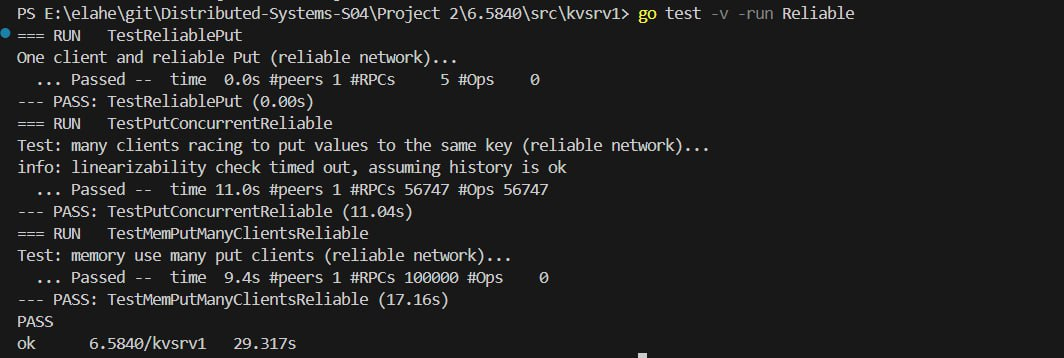
\includegraphics[width=0.85\linewidth]{Template - Student/Content/1.jpg}
\caption{خروجی نتایج تست‌های سرویس کلید/مقدار در شرایط شبکه قابل اطمینان (بدون فلگ \lr{race})}
\label{fig:reliable-test-results}
\end{figure}

\begin{figure}[H]
\centering
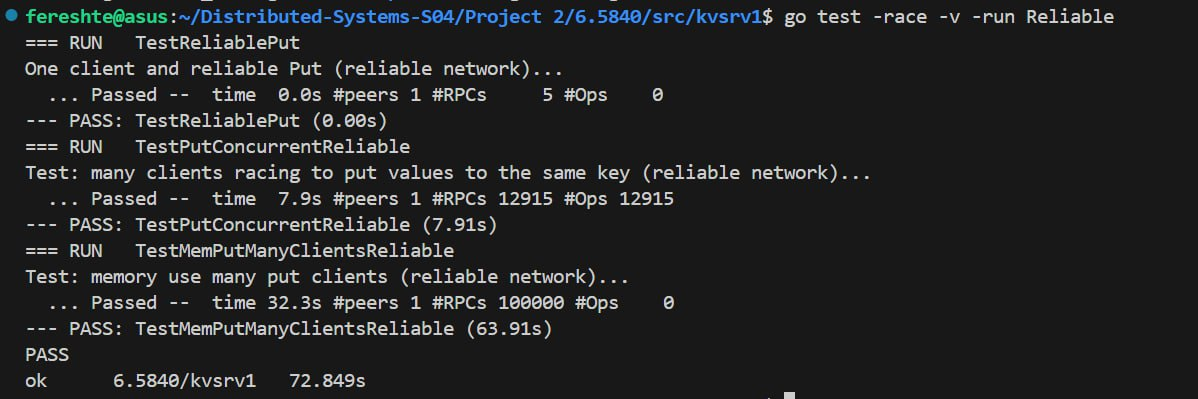
\includegraphics[width=0.85\linewidth]{Template - Student/Content/1_race.jpg}
\caption{خروجی نتایج تست‌های سرویس کلید/مقدار در شرایط شبکه قابل اطمینان (با فلگ \lr{race})}
\label{fig:reliable-test-results-race}
\end{figure}

\begin{figure}[H]
\centering
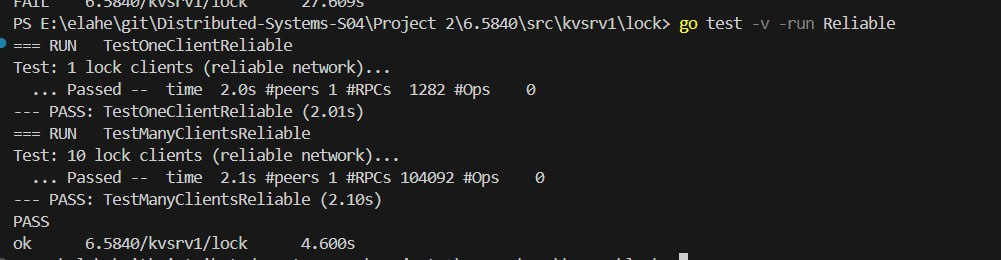
\includegraphics[width=0.85\linewidth]{Template - Student/Content/2.jpg}
\caption{خروجی نتایج تست‌های سرویس کلید/مقدار در شرایط شبکه ناپایدار (بدون فلگ \lr{race})}
\label{fig:unreliable-test-results}
\end{figure}

\begin{figure}[H]
\centering
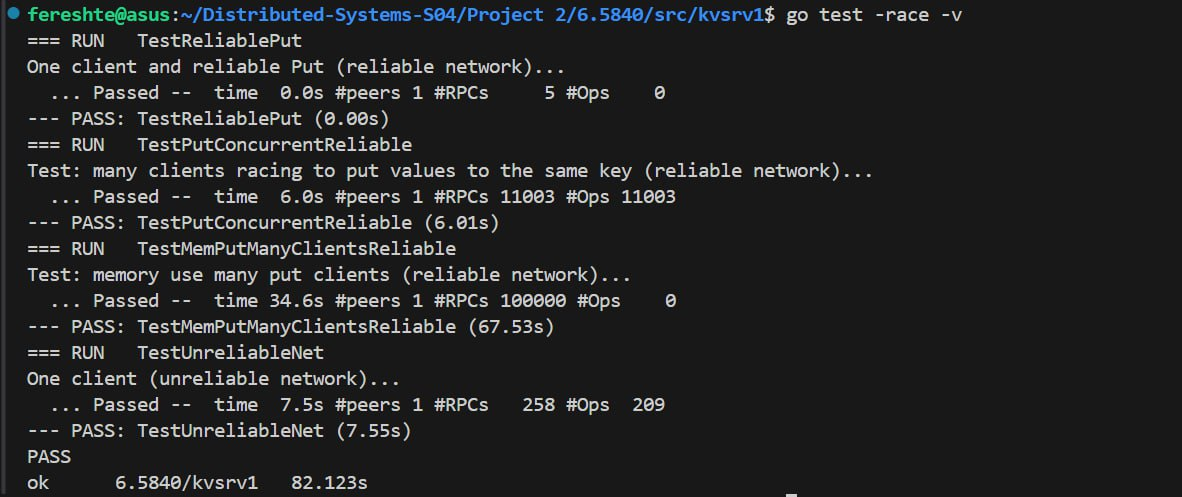
\includegraphics[width=0.85\linewidth]{Template - Student/Content/2_race.jpg}
\caption{خروجی نتایج تست‌های سرویس کلید/مقدار در شرایط شبکه ناپایدار (با فلگ \lr{race})}
\label{fig:unreliable-test-results-race}
\end{figure}

\begin{figure}[H]
\centering
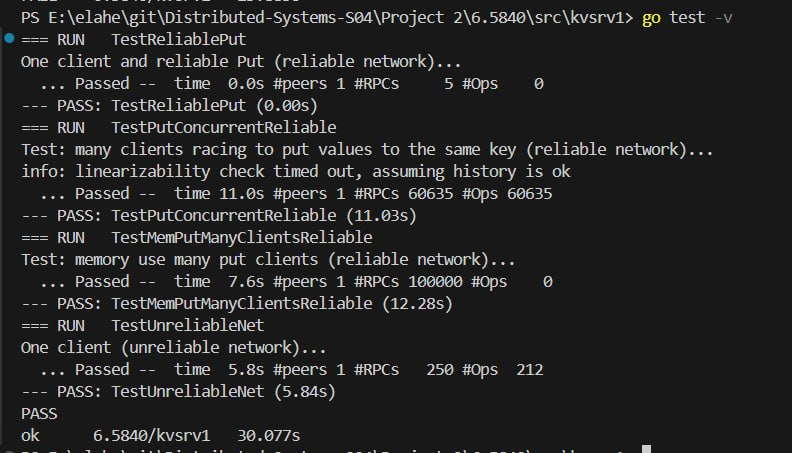
\includegraphics[width=0.85\linewidth]{Template - Student/Content/3.jpg}
\caption{خروجی نتایج تست‌های قفل توزیع‌شده در شرایط شبکه قابل اطمینان (بدون فلگ \lr{race})}
\label{fig:lock-reliable-test-results}
\end{figure}

\begin{figure}[H]
\centering
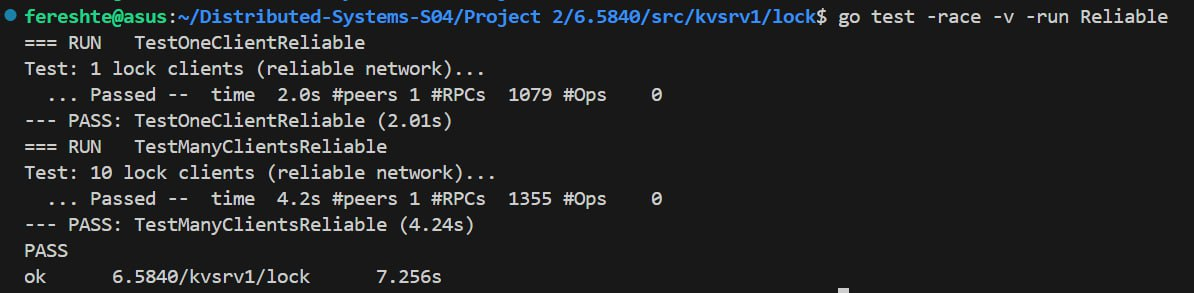
\includegraphics[width=0.85\linewidth]{Template - Student/Content/3_race.jpg}
\caption{خروجی نتایج تست‌های قفل توزیع‌شده در شرایط شبکه قابل اطمینان (با فلگ \lr{race})}
\label{fig:lock-reliable-test-results-race}
\end{figure}

\begin{figure}[H]
\centering
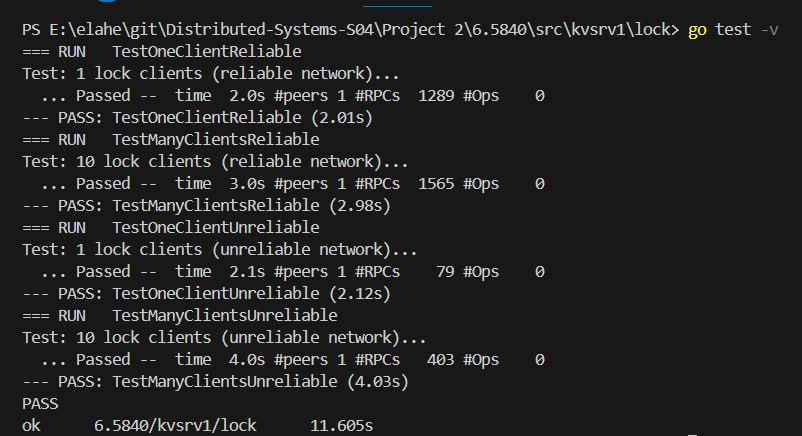
\includegraphics[width=0.85\linewidth]{Template - Student/Content/4.jpg}
\caption{خروجی نتایج تست‌های قفل توزیع‌شده در شرایط شبکه ناپایدار (بدون فلگ \lr{race})}
\label{fig:lock-unreliable-test-results}
\end{figure}

\begin{figure}[H]
\centering
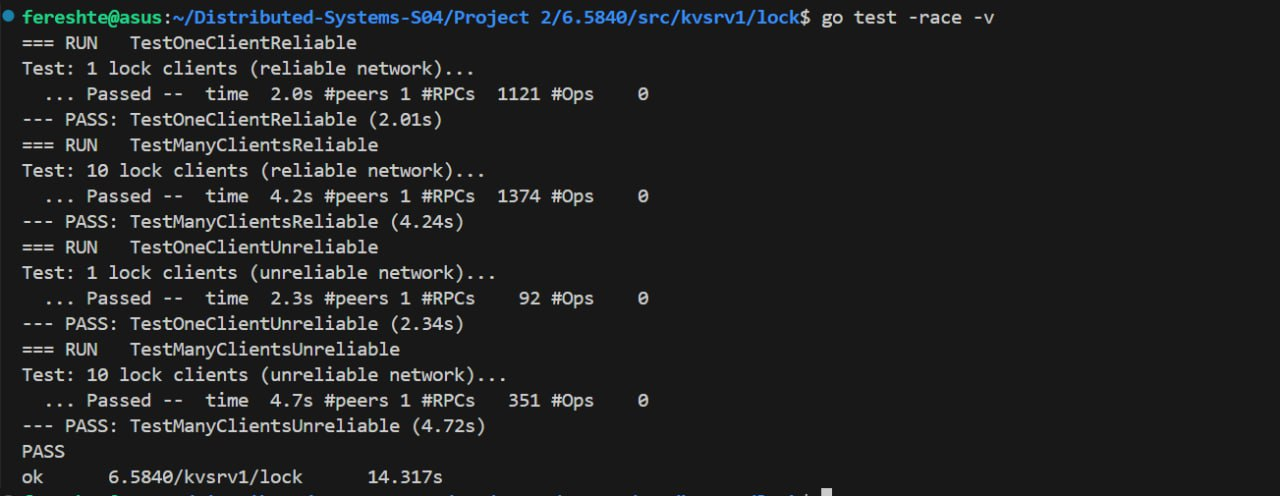
\includegraphics[width=0.85\linewidth]{Template - Student/Content/4_race.jpg}
\caption{خروجی نتایج تست‌های قفل توزیع‌شده در شرایط شبکه ناپایدار (با فلگ \lr{race})}
\label{fig:lock-unreliable-test-results-race}
\end{figure}

\subsection*{نتیجه‌گیری}

پس از اجرای تمام تست‌ها، نتایج نشان داد که سیستم به درستی در شرایط مختلف شبکه عمل می‌کند:
\begin{itemize}
    \item در شرایط شبکه قابل اطمینان، سیستم به‌طور صحیح داده‌ها را ذخیره و بازیابی کرده و قفل‌ها به درستی بین کلاینت‌ها توزیع شدند.
    \item در شرایط ناپایدار شبکه، سیستم توانست با استفاده از مکانیزم \texttt{retry} و \texttt{backoff} به درستی از مشکلات ناشی از گم شدن پیام‌ها و تأخیرها جلوگیری کند و عملکرد خود را حفظ کند.
    \item تست‌های قفل توزیع‌شده نشان داد که سیستم قادر است به‌طور ایمن دسترسی به منابع مشترک را مدیریت کرده و از تداخل در دسترسی‌های همزمان جلوگیری کند.
\end{itemize}

این تست‌ها به‌ویژه در ارزیابی رفتار سیستم در شرایط مختلف شبکه و شبیه‌سازی شرایط واقعی شبکه مفید بودند. با استفاده از این تست‌ها، به‌طور دقیق از صحت عملکرد سیستم در شرایط مختلف اطمینان حاصل کردیم و توانستیم نقاط قوت و ضعف سیستم را شناسایی کنیم. در نهایت، سیستم طراحی‌شده قادر است در برابر چالش‌های محیط‌های ناپایدار شبکه به‌طور موثر عمل کند.


\end{document}